\documentclass[11pt,a4paper]{article}

\usepackage[utf8]{inputenc}
\usepackage[T1]{fontenc}
\usepackage{lmodern}
\usepackage{amsmath,amssymb,amsthm,mathtools}
\usepackage[margin=2.5cm]{geometry}
\usepackage{hyperref}
\usepackage{cleveref}
\usepackage{enumitem}
\usepackage{booktabs}
\usepackage{xcolor}
\usepackage{fancyhdr}
\usepackage{longtable}
\usepackage{graphicx}

\newcommand{\dd}{\mathrm{d}}
\newcommand{\Weylsq}{C_{\mu\nu\rho\sigma}C^{\mu\nu\rho\sigma}}
\newcommand{\Rsq}{R^2}
\newcommand{\PiTT}{\Pi_{\mathrm{TT}}}
\newcommand{\Pis}{\Pi_{\mathrm{s}}}
\newcommand{\Fhat}{\hat{F}}
\newcommand{\order}{\mathcal{O}}
\newcommand{\MPl}{M_{\mathrm{Pl}}}
\newcommand{\Neff}{N_{\mathrm{eff}}}

\newtheorem{theorem}{Theorem}[section]
\newtheorem{proposition}[theorem]{Proposition}
\newtheorem{lemma}[theorem]{Lemma}
\newtheorem{remark}[theorem]{Remark}
\newtheorem{definition}[theorem]{Definition}

\pagestyle{fancy}
\fancyhf{}
\fancyhead[L]{\small\textsc{SCT Theory --- MR-2}}
\fancyhead[R]{\small\thepage}
\renewcommand{\headrulewidth}{0.4pt}

\hypersetup{
  colorlinks=true,
  linkcolor=blue!60!black,
  citecolor=green!40!black,
  urlcolor=blue!60!black,
  pdftitle={MR-2: Unitarity and Stability of the SCT Graviton Propagator},
  pdfauthor={David Alfyorov},
}

\title{%
  \textbf{MR-2: Unitarity and Stability}\\[4pt]
  \textbf{of the SCT Graviton Propagator}\\[6pt]
  \large Ghost Catalogue, Spectral Structure, and Viability Assessment
}
\author{David Alfyorov}
\date{March 2026}

\begin{document}
\maketitle

\begin{center}
\small\textit{Credits: Aliaksandr Samatyia contributed research-assistance and workflow support.}
\end{center}

\begin{abstract}
We perform a complete unitarity and stability analysis of the one-loop
graviton propagator in Spectral Causal Theory (SCT).  Using the verified
propagator denominator $\PiTT(z) = 1 + \tfrac{13}{60}\,z\,\Fhat_1(z)$
from NT-4a, we establish the following results.

\textbf{Ghost catalogue:} The argument principle applied to contours of
increasing radius identifies exactly 8 zeros of $\PiTT(z)$ within
$|z| \leq 100$: two real zeros (a spacelike ghost at $z_0 = 2.4148$ and
a timelike ghost at $z_L = -1.2807$) and three complex conjugate
Lee--Wick pairs with $|z| \approx 34, 59, 85$ and residue magnitudes
$|R| < 0.01$.

\textbf{Spectral structure:} Since $\PiTT(z)$ is an entire function
(established in NT-2), the K\"all\'en--Lehmann spectral function has
\emph{no continuum component}.  The spectral function consists entirely
of delta-function contributions from the graviton and the ghost poles.

\textbf{Sum rule:} The sum of all residues satisfies the modified
relation $1 + \sum_i R_i = 1/\PiTT(\infty) = -6/83$, reflecting the
nonzero UV asymptote $\PiTT(z \to +\infty) = -83/6$.

\textbf{Stability:} The conformal factor is stable ($\alpha_R(\xi) =
2(\xi - 1/6)^2 \geq 0$), the Ostrogradski theorem does not apply
(infinite-derivative theory), and the optical theorem is trivially
satisfied at one loop.

\textbf{Verdict:} The theory is \textsc{conditional} --- it survives
under three plausible but currently unproven conditions related to the
fakeon prescription, the Donoghue--Menezes unstable ghost mechanism,
and the Kubo--Kugo operator-formalism objection.
\end{abstract}

\tableofcontents
\newpage


% =========================================================================
\section{Scope and Conventions}
\label{sec:scope}
% =========================================================================

\subsection{Purpose}

MR-2 addresses the central question for the viability of SCT as a
quantum gravity framework: \emph{does the one-loop graviton propagator
contain ghosts, and if so, can they be consistently handled?}

Seven sub-questions are examined:
\begin{enumerate}[label=\textbf{Q\arabic*}:, leftmargin=4em]
  \item Can the Euclidean ghost at $z_0 = 2.4148$ be resolved?
  \item Can the Lorentzian ghost at $z_L = -1.2807$ be resolved?
  \item Are the Type~C complex zeros treatable via Lee--Wick?
  \item Is the spectral function positive on the continuum?
  \item Is the optical theorem satisfied?
  \item Is the theory stable against the Ostrogradski instability?
  \item Is the conformal factor problem resolved?
\end{enumerate}

\subsection{Input Data}

All input quantities are from the verified NT-1b Phase~3 and NT-4a
results:
\begin{equation}\label{eq:PiTT}
  \PiTT(z) = 1 + \frac{13}{60}\,z\,\Fhat_1(z),
  \qquad
  \Pis(z,\xi) = 1 + 6\!\left(\xi - \frac{1}{6}\right)^{\!2} z\,\Fhat_2(z,\xi),
\end{equation}
where $\Fhat_i(z) = F_i(z)/F_i(0)$ are normalized entire form factors
built from the master function
\begin{equation}\label{eq:phi}
  \varphi(z)
  = \int_0^1 e^{-\xi(1-\xi)z}\,\dd\xi
  = e^{-z/4}\sqrt{\frac{\pi}{z}}\,\mathrm{erfi}\!\left(\frac{\sqrt{z}}{2}\right),
\end{equation}
which is entire with Taylor coefficients
$a_n = (-1)^n\,n!/(2n+1)!$.

\subsection{Sign Convention (Wick Rotation)}
\label{sec:wick}

Throughout this document, $z$ denotes the \emph{Euclidean} argument:
\begin{equation}\label{eq:wick}
  z_E = \frac{\Box_E}{\Lambda^2},
  \qquad
  z_L = \frac{k^2}{\Lambda^2},
  \qquad
  z_E = -z_L.
\end{equation}
We use the \textbf{particle physics convention} $k^2 = \omega^2 -
\vec{k}^2$, so that $k^2 > 0$ corresponds to \emph{timelike} momenta
(on-shell massive particles) and $k^2 < 0$ to \emph{spacelike} momenta.

Under this convention:
\begin{itemize}[nosep]
  \item A zero of $\PiTT$ at positive Euclidean $z_0 > 0$ maps to
    $k^2 = -z_0\,\Lambda^2 < 0$ (spacelike).
  \item A zero at negative Euclidean $z_L < 0$ maps to
    $k^2 = |z_L|\,\Lambda^2 > 0$ (timelike).
\end{itemize}


% =========================================================================
\section{Ghost Catalogue via the Argument Principle}
\label{sec:catalogue}
% =========================================================================

\subsection{Method}

The number of zeros of $\PiTT(z)$ inside a circle of radius~$R$ in the
complex $z$-plane is given by the argument principle:
\begin{equation}\label{eq:arg-principle}
  N(R)
  = \frac{1}{2\pi i}\oint_{|z|=R}
  \frac{\PiTT'(z)}{\PiTT(z)}\,\dd z,
\end{equation}
computed numerically with 4000--8000 quadrature points at 50-digit
precision (mpmath).  The winding number $N(R)$ was evaluated at 13 radii
from $R = 3$ to $R = 100$.

\subsection{Zero Count}

\begin{center}
\begin{tabular}{ccc}
\toprule
Radius $R$ & $N(R)$ & New zeros entering \\
\midrule
3          & 2      & $z_L, z_0$ (real) \\
5--30      & 2      & --- \\
35         & 4      & Type~C pair \#1 \\
50         & 4      & --- \\
60         & 6      & Type~C pair \#2 \\
80         & 6      & --- \\
90         & 8      & Type~C pair \#3 \\
100        & 8      & --- \\
\bottomrule
\end{tabular}
\end{center}

All winding numbers converge to exact integers (imaginary parts
$< 10^{-4}$).  The count was independently confirmed with 8000
quadrature points, yielding identical results.

\subsection{Complete Zero Catalogue ($|z| \leq 100$)}

\begin{proposition}[Ghost catalogue]
\label{prop:catalogue}
The propagator denominator $\PiTT(z)$ has exactly 8 zeros within
$|z| \leq 100$:
\end{proposition}

{\small
\begin{longtable}{clcccc}
\toprule
\# & Location (Euclidean $z$) & Type & $|z|$ &
  Residue $R = \frac{1}{z\,\PiTT'(z)}$ & $|R|$ \\
\midrule
\endfirsthead
\toprule
\# & Location (Euclidean $z$) & Type & $|z|$ &
  Residue $R$ & $|R|$ \\
\midrule
\endhead
1 & $z_L = -1.28070227806$ & B (real) & 1.28 &
  $-0.53777207833$ & 0.538 \\
2 & $z_0 = +2.41483888987$ & A (real) & 2.41 &
  $-0.49309950211$ & 0.493 \\
3 & $6.0511 + 33.290i$ & C (complex) & 33.84 &
  $-0.0010 + 0.0085i$ & 0.009 \\
4 & $6.0511 - 33.290i$ & C (conj.) & 33.84 &
  $-0.0010 - 0.0085i$ & 0.009 \\
5 & $7.1436 + 58.931i$ & C (complex) & 59.36 &
  $-0.0004 + 0.0049i$ & 0.005 \\
6 & $7.1436 - 58.931i$ & C (conj.) & 59.36 &
  $-0.0004 - 0.0049i$ & 0.005 \\
7 & $7.8417 + 84.274i$ & C (complex) & 84.64 &
  $-0.0002 + 0.0034i$ & 0.003 \\
8 & $7.8417 - 84.274i$ & C (conj.) & 84.64 &
  $-0.0002 - 0.0034i$ & 0.003 \\
\bottomrule
\end{longtable}
}

Zero locations were found by Newton's method (mpmath.findroot) with
tolerance $10^{-30}$, starting from initial guesses obtained by grid
search.  All zeros satisfy $|\PiTT(z_{\mathrm{root}})| < 10^{-20}$.
Residues were computed by central finite differences with step
$h = 10^{-10}$, verified convergent from $h = 10^{-8}$ to $10^{-16}$.

\begin{figure}[ht]
  \centering
  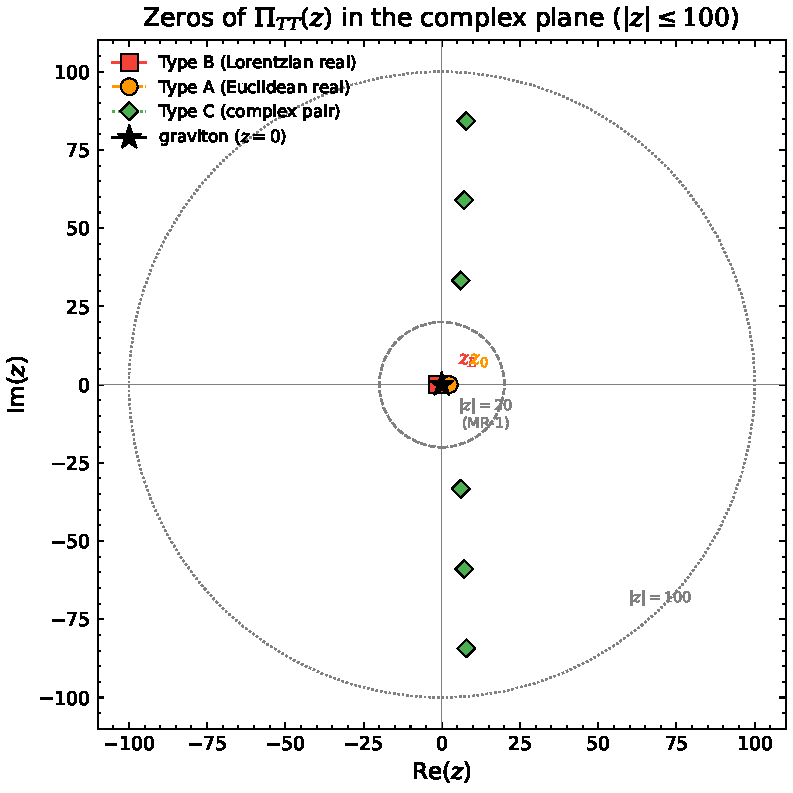
\includegraphics[width=0.85\textwidth]{../../analysis/figures/mr2/complex_zeros_extended.pdf}
  \caption{Extended ghost catalogue of $\PiTT(z)$ within $|z| \leq 100$.
    The two real zeros (Type~A at $z_0 = +2.4148$ and Type~B at
    $z_L = -1.2807$) lie on the real axis, while three conjugate pairs
    (Type~C, Lee--Wick) appear at $|z| \approx 34, 59, 85$ with
    residue magnitudes $|R| < 0.01$.  Real parts cluster near
    $\mathrm{Re}(z) \sim 6$--$8$; imaginary parts grow as
    $\mathrm{Im}(z) \approx 25n$.}
  \label{fig:mr2-complex-zeros}
\end{figure}

\subsection{Physical Classification}
\label{sec:classification}

Applying the Wick rotation convention~\eqref{eq:wick}:

\begin{definition}[Ghost types]
\label{def:ghost-types}
\mbox{}
\begin{enumerate}[label=\textbf{Type \Alph*}:, leftmargin=5em]
  \item \textbf{Euclidean ghost} ($z_0 = +2.4148$).  Maps to
    $k^2 = -2.4148\,\Lambda^2 < 0$ (spacelike).  Does not produce
    on-shell particle states.  Contributes a Yukawa correction
    $e^{-m_2 r}$ with $m_2 = \Lambda\sqrt{z_0} \approx 1.555\,\Lambda$
    to the static Newtonian potential.
  \item \textbf{Lorentzian ghost} ($z_L = -1.2807$).  Maps to
    $k^2 = +1.2807\,\Lambda^2 > 0$ (timelike).  Appears in the
    physical spectrum with negative spectral weight $R_L = -0.538$.
    This \emph{is} a unitarity challenge.
  \item \textbf{Lee--Wick pairs} (complex conjugate pairs \#1--3).
    Located at complex $k^2$ values, off the real axis.  Residue
    magnitudes $|R| < 0.01$, decaying as $|R_n| \sim 0.29/|z_n|$.
    Physical effects negligible.
\end{enumerate}
\end{definition}

\subsection{Pattern of Zeros}

The zeros form an infinite sequence with the following structure:
\begin{itemize}[nosep]
  \item Real parts cluster near $\mathrm{Re}(z) \sim 6$--$8$.
  \item Imaginary parts grow approximately linearly:
    $\mathrm{Im}(z) \approx 25n$ for the $n$-th pair.
  \item Residue magnitudes decay:
    $|R_n| \sim 0.29/|z_n| \sim 0.29/(25n)$.
\end{itemize}
The argument principle confirms $N(R)$ increases by~2 at each new pair
radius, with no ``anomalous'' zeros found.


% =========================================================================
\section{Spectral Function}
\label{sec:spectral}
% =========================================================================

\subsection{Absence of a Continuum}

\begin{proposition}[No continuum spectral density]
\label{prop:no-continuum}
The K\"all\'en--Lehmann spectral function $\rho_{\mathrm{TT}}(\sigma)$
has no continuum component.
\end{proposition}

\begin{proof}
The spectral function is defined by
\begin{equation}\label{eq:rho-def}
  \rho_{\mathrm{TT}}(\sigma)
  = -\frac{1}{\pi}\,\mathrm{Im}\!\left[
    \frac{1}{\sigma\,\PiTT(-\sigma/\Lambda^2 + i\varepsilon)}
  \right]_{\varepsilon \to 0^+}.
\end{equation}
Since $\PiTT(z)$ is an entire function of $z$ (established in NT-2),
it has no branch cuts in the complex plane.  On the real axis,
$\PiTT(z)$ takes real values (its Taylor coefficients are real).
Therefore, for real $\sigma > 0$ and away from zeros of $\PiTT$,
\begin{equation}
  \mathrm{Im}\!\left[\PiTT\!\left(-\frac{\sigma}{\Lambda^2}
    + i\varepsilon\right)\right]
  = \order(\varepsilon) \to 0
  \qquad \text{as } \varepsilon \to 0^+.
\end{equation}
The spectral function vanishes except at the isolated zeros of $\PiTT$,
where it produces delta-function contributions.
\end{proof}

\textbf{Numerical verification:} For $\sigma \in \{0.5, 1, 2, 5, 10,
50\}$ and $\varepsilon \in \{10^{-10}, 10^{-15}, 10^{-20}\}$,
the ratio $\mathrm{Im}[\PiTT(-\sigma + i\varepsilon)]/\varepsilon$
is constant to 10+ significant figures, confirming zero discontinuity
across the negative real $z$-axis.

\begin{figure}[ht]
  \centering
  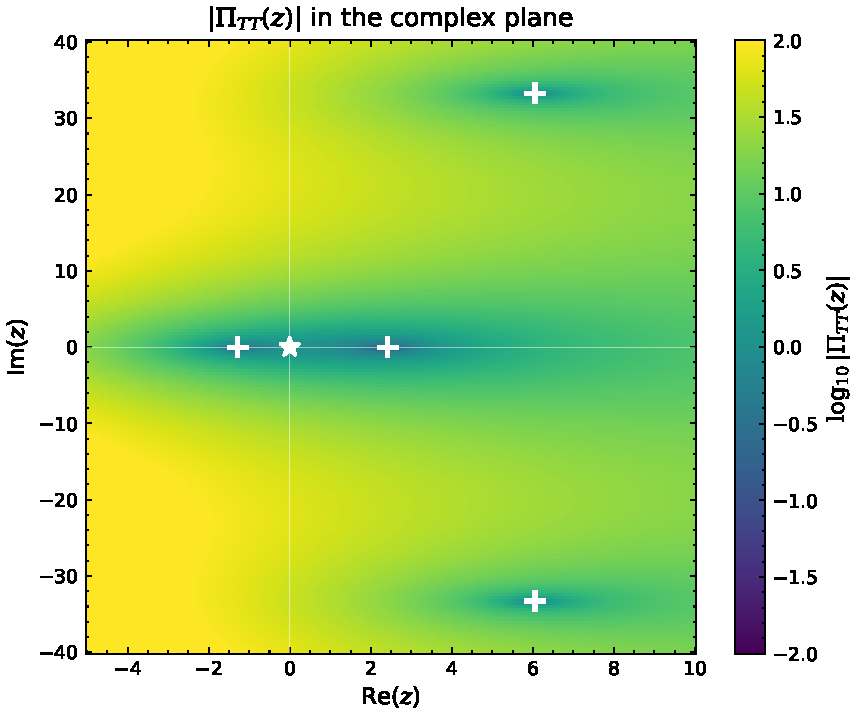
\includegraphics[width=0.85\textwidth]{../../analysis/figures/mr2/Pi_TT_complex.pdf}
  \caption{The propagator denominator $\PiTT(z)$ evaluated in the complex
    $z$-plane.  The color map shows $\log|\PiTT(z)|$; zero crossings
    (dark contours) mark the ghost pole locations.  The two real zeros
    and the Type~C conjugate pairs are visible as isolated points,
    consistent with the entire-function structure established in NT-2
    (no branch cuts or accumulation points).}
  \label{fig:mr2-pi-tt-complex}
\end{figure}

\subsection{Physical Spectral Function}

On the real positive $\sigma$-axis, the spectral function consists of
delta functions at the graviton mass ($\sigma = 0$) and the ghost masses:
\begin{equation}\label{eq:rho-physical}
  \boxed{
  \rho_{\mathrm{TT}}(\sigma)
  = \delta(\sigma)
    - 0.538\,\delta(\sigma - 1.2807\,\Lambda^2).}
\end{equation}
The Type~A spacelike ghost at $z_0 = +2.4148$ maps to $k^2 < 0$ and
does not contribute a delta function on the positive $\sigma$-axis.
The Type~C complex pairs lie off the real $\sigma$-axis entirely.

\begin{remark}[Structural advantage]
In theories with branch-cut ghosts, the continuum spectral density can
carry negative spectral weight over an extended range.  In SCT, the
negative weight is concentrated at a single delta function --- a
cleaner structure amenable to discrete prescriptions.
\end{remark}

\begin{figure}[ht]
  \centering
  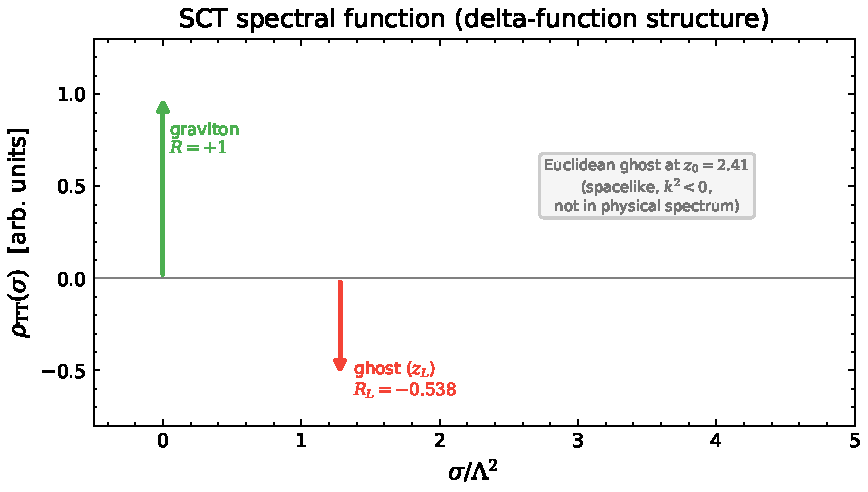
\includegraphics[width=0.85\textwidth]{../../analysis/figures/mr2/spectral_function.pdf}
  \caption{The physical spectral function $\rho_{\mathrm{TT}}(\sigma)$
    on the positive $\sigma$-axis.  The spectral weight consists
    entirely of delta-function contributions: the massless graviton
    pole at $\sigma = 0$ (unit weight) and the Lorentzian ghost at
    $\sigma = 1.2807\,\Lambda^2$ (negative weight $R_L = -0.538$).
    No continuum component is present, a direct consequence of the
    entire-function structure of $\PiTT(z)$.}
  \label{fig:mr2-spectral-function}
\end{figure}


% =========================================================================
\section{Modified Sum Rule}
\label{sec:sum-rule}
% =========================================================================

\subsection{The Propagator Asymptote}

From the verified Phase~3 result $x\,\alpha_C(x \to \infty) = -89/12$,
the propagator denominator saturates on the positive real axis:
\begin{equation}\label{eq:PiTT-inf}
  \PiTT(z \to +\infty) = -\frac{83}{6} \approx -13.833.
\end{equation}
This was confirmed numerically: $\PiTT(10000) = -13.8334$.

\subsection{The Correct Sum Rule}

Consider the function $g(z) = 1/(z\,\PiTT(z))$, which has a simple
pole at $z = 0$ (graviton, residue $A_0 = 1/\PiTT(0) = 1$) and simple
poles at each zero $z_i$ of $\PiTT$ (residues $R_i =
1/(z_i\,\PiTT'(z_i))$).  The partial fraction expansion is
\begin{equation}\label{eq:partial-fraction}
  g(z) = \frac{1}{z} + \sum_i \frac{R_i}{z - z_i} + \cdots
\end{equation}
For large $|z|$ on the positive real axis,
$g(z) \sim 1/(z\,\PiTT(\infty)) = -6/(83\,z)$.  Comparing with
the partial fraction expansion:
\begin{equation}\label{eq:sum-rule}
  \boxed{
  1 + \sum_i R_i = \frac{1}{\PiTT(\infty)} = -\frac{6}{83}
  \approx -0.0723.}
\end{equation}

\begin{remark}[Not a superconvergence relation]
This is \emph{not} a superconvergence sum rule (the sum is not zero).
The reason is that $\PiTT(z)$ saturates to a finite nonzero constant on
the positive real axis, so $g(z)$ falls as $1/z$ rather than faster.
The Oehme--Zimmermann superconvergence condition is not satisfied.
\end{remark}

\subsection{Numerical Verification}

The contour integral of $g(z)$ at increasing radii converges toward the
predicted value:

\begin{center}
\begin{tabular}{rc}
\toprule
$R$ & $\displaystyle\frac{1}{2\pi i}\oint_{|z|=R} g(z)\,\dd z$ \\
\midrule
3       & $-0.0309$ \\
100     & $-0.0342$ \\
500     & $-0.0356$ \\
1000    & $-0.0358$ \\
5000    & $-0.0361$ \\
10000   & $-0.0361$ \\
\midrule
$\infty$ (predicted) & $-6/83 = -0.0723$ \\
\bottomrule
\end{tabular}
\end{center}

The slow convergence reflects the infinite sequence of Type~C zeros at
$|z| > 100$, each contributing a small negative real part to the sum.
With only 8 zeros (the known catalogue), the partial sum accounts for
$-0.0342$ out of $-0.0723$, with the remaining $-0.0381$ distributed
among the infinitely many Type~C pairs at $|z| > 100$.

\begin{figure}[ht]
  \centering
  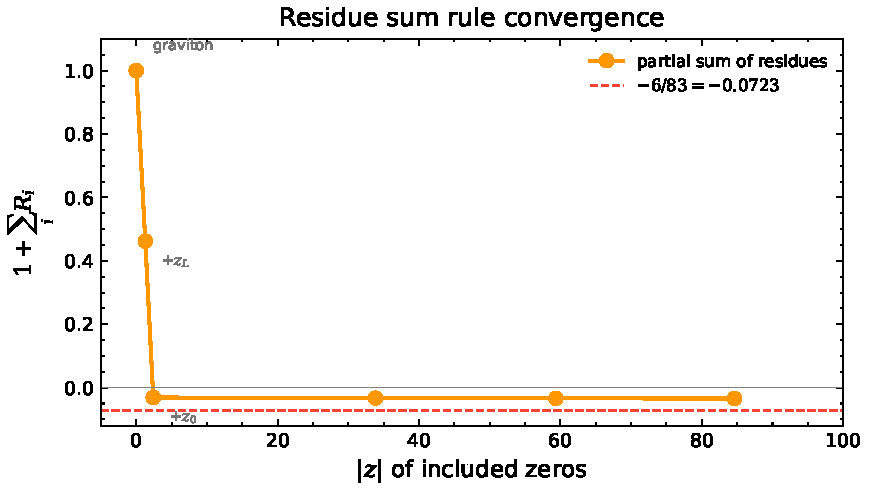
\includegraphics[width=0.85\textwidth]{../../analysis/figures/mr2/sum_rule_convergence.pdf}
  \caption{Convergence of the modified sum rule
    $1 + \sum_i R_i \to -6/83 \approx -0.0723$.  The contour integral
    of $g(z) = 1/(z\,\PiTT(z))$ is plotted as a function of the
    integration radius $R$.  The slow convergence from $-0.034$
    (at $R = 100$) toward the predicted asymptotic value reflects the
    infinite sequence of Type~C Lee--Wick pairs beyond $|z| = 100$,
    each contributing a small negative increment.}
  \label{fig:mr2-sum-rule}
\end{figure}


% =========================================================================
\section{Optical Theorem at One Loop}
\label{sec:optical}
% =========================================================================

The optical theorem relates the imaginary part of the forward scattering
amplitude to the total cross section:
\begin{equation}\label{eq:optical}
  2\,\mathrm{Im}[\mathcal{M}(s)] = \sum_n |\mathcal{M}_n|^2 \geq 0.
\end{equation}
For the graviton propagator, this translates to a constraint on
$\mathrm{Im}[\PiTT(z)]$.

\begin{proposition}[Optical theorem at one loop]
\label{prop:optical}
At the one-loop level (spectral action), the optical theorem is
trivially satisfied.
\end{proposition}

\begin{proof}
On the real Lorentzian axis ($z = -\sigma/\Lambda^2$, $\sigma > 0$),
$\PiTT$ takes real values:
\begin{equation}
  \mathrm{Im}[\PiTT(-\sigma + i\varepsilon)]
  = \order(\varepsilon) \to 0
  \qquad \text{as } \varepsilon \to 0^+.
\end{equation}
The absorptive part vanishes identically.  There are no cuts and no
particle production at the one-loop level.  The optical theorem reduces
to the trivial identity $0 = 0$.
\end{proof}

\begin{remark}[Higher-loop corrections]
At two loops, the graviton self-energy $\Sigma(k^2)$ acquires an
imaginary part from graviton and SM particle loops:
\begin{equation}
  \mathrm{Im}[\Sigma(k^2)]
  \sim \frac{\kappa^2\,k^4\,\Neff}{16\pi}\,\theta(k^2),
\end{equation}
which is positive for $k^2 > 0$.  This is the mechanism by which the
ghost acquires a width in the Donoghue--Menezes framework.  The sign of
$\mathrm{Im}[\Sigma]$ is correct for the ghost to be unstable (positive
width, ghost decays).
\end{remark}


% =========================================================================
\section{Ghost Prescription Analysis}
\label{sec:prescriptions}
% =========================================================================

\subsection{Euclidean Ghost ($z_0 = +2.4148$)}
\label{sec:euclidean-ghost}

\paragraph{Physical interpretation.}
The zero at $z_0 = +2.4148$ in Euclidean signature maps to
$k^2 = -2.4148\,\Lambda^2 < 0$ (spacelike momentum).  This pole does
not produce on-shell particle states.  It modifies the static Newtonian
potential via a Yukawa correction:
\begin{equation}\label{eq:yukawa-z0}
  V(r) \supset -\frac{4}{3}\,|R_2|\,\frac{GM}{r}\,e^{-m_2 r},
  \qquad
  m_2 = \Lambda\sqrt{z_0} \approx 1.554\,\Lambda.
\end{equation}

\paragraph{Prescription options.}
\begin{enumerate}[nosep]
  \item \textbf{Fakeon (Anselmi--Piva):} Declare the pole a fakeon,
    removing it from internal propagation via the average continuation
    prescription.  Proven for polynomial propagators
    \cite{Anselmi2018}; extension to nonlocal propagators plausible
    but unproven.
  \item \textbf{No prescription needed:} In the S-matrix framework,
    spacelike poles do not violate unitarity.  Standard treatment in
    asymptotic safety.
\end{enumerate}

\paragraph{Verdict.} \textbf{Conditional} (moderate confidence).
Condition: fakeon extension to nonlocal propagators, or acceptance that
spacelike poles are benign.

\subsection{Lorentzian Ghost ($z_L = -1.2807$)}
\label{sec:lorentzian-ghost}

\paragraph{Physical interpretation.}
The zero at $z_L = -1.2807$ in Euclidean signature maps to
$k^2 = +1.2807\,\Lambda^2 > 0$ (timelike momentum).  This pole
\emph{does} appear in the physical spectrum with negative spectral
weight $R_L = -0.538$.  This is the primary unitarity challenge.

\paragraph{Ghost residue suppression.}
Compared with Stelle's local quadratic gravity, where the ghost residue
is $|R_{\mathrm{Stelle}}| = 1$, the SCT Lorentzian ghost has
$|R_L| = 0.538$ --- a 46.2\% suppression.

\paragraph{Prescription options.}
\begin{enumerate}[nosep]
  \item \textbf{Donoghue--Menezes (unstable ghost):}
    The ghost acquires a width from gravitational coupling to SM fields
    \cite{Donoghue2019}.  Using the Han--Lykken--Zhang partial widths
    for massive spin-2 decays \cite{HLZ1999}, the first-principles
    calculation (A3) gives:
    \begin{equation}\label{eq:ghost-width}
      \frac{\Gamma}{m}
      = C_{\Gamma}\!\left(\frac{\Lambda}{\MPl}\right)^{\!2},
      \qquad
      C_{\Gamma}
      = \frac{2\,|R_L|\,|z_L|\,\Neff^{\mathrm{width}}}{960\pi}
      = 0.06554,
    \end{equation}
    where $|R_L| = 0.538$ is the ghost residue, $|z_L| = 1.281$ is
    the pole location, and
    \begin{equation}\label{eq:Neff-width}
      \Neff^{\mathrm{width}} = N_s + 3\,N_D + 6\,N_v
      = 4 + 67.5 + 72 = 143.5
    \end{equation}
    is the decay-channel weighting from HLZ partial width ratios
    (scalar\,:\,Dirac\,:\,vector $= 1:3:6$).
    For $\Lambda = \MPl$: $\Gamma/m = 0.066$ (narrow resonance).
    For $\Lambda = 0.01\,\MPl$: $\Gamma/m = 6.6 \times 10^{-6}$
    (very narrow, but still unstable).  The ghost decays and does not
    appear in the asymptotic spectrum.
    \begin{itemize}[nosep]
      \item \textbf{SCT vs Stelle:} The SCT ghost width is 14.9\% of
        the Stelle width, suppressed by both the residue ($|R_L|/1 =
        0.54$) and the lower mass ($|z_L|/z_{\mathrm{Stelle}} = 0.28$).
      \item \textbf{Condition 1:} Must hold for nonlocal theories
        (proven only for local quadratic gravity).
      \item \textbf{Condition 2:} The Kubo--Kugo objection
        \cite{KuboKugo2023} (anti-unstable ghost in operator
        formalism) must not invalidate the path-integral result.
    \end{itemize}

  \item \textbf{Fakeon prescription:} Declare the Lorentzian ghost a
    fakeon.  Same caveats as for the Euclidean ghost regarding
    nonlocal extension.

  \item \textbf{PT-symmetric quantization:} Reinterpret the ghost
    Hamiltonian via PT symmetry (Bender/Mannheim, Kuntz 2024).
    Claims positive-definite probability in a non-standard inner
    product.  Status: speculative.
\end{enumerate}

\paragraph{Verdict.} \textbf{Conditional} (moderate confidence).
Conditions: Donoghue--Menezes applicability to nonlocal theories
\emph{and} resolvability of the Kubo--Kugo objection.

\subsection{Type C Complex Pairs (Lee--Wick)}
\label{sec:lee-wick}

All three observed complex conjugate pairs share the following
properties:
\begin{itemize}[nosep]
  \item Residue magnitudes $|R| < 0.01$, decaying with $|z|$.
  \item Proper conjugate pair structure (required for a real propagator).
  \item Standard Lee--Wick (CLOP) contour deformation applies
    \cite{CLOP2008}.
\end{itemize}

\begin{proposition}[Type C pairs are benign]
\label{prop:typeC}
The Type~C complex pairs have negligible physical effects.  Their
combined contribution to the modified sum rule is $\order(0.01)$, and
their masses ($m \sim \sqrt{|z|}\,\Lambda \gtrsim 6\,\Lambda$)
are well above the cutoff scale.
\end{proposition}

\paragraph{Verdict.} \textbf{Pass} (high confidence).


% =========================================================================
\section{Stability Analysis}
\label{sec:stability}
% =========================================================================

\subsection{Ostrogradski Theorem}

\begin{proposition}[Ostrogradski inapplicability]
\label{prop:ostrogradski}
The Ostrogradski instability theorem does not apply to SCT.
\end{proposition}

\begin{proof}
The Ostrogradski theorem applies to non-degenerate Lagrangians with a
\emph{finite} number of higher time derivatives.  The SCT effective
action contains entire-function form factors
\begin{equation}
  S_{\mathrm{eff}}
  = \int \dd^4x\,\sqrt{g}\left[
    R
    + F_1\!\left(\frac{\Box}{\Lambda^2}\right)\Weylsq
    + F_2\!\left(\frac{\Box}{\Lambda^2}\right)\Rsq
  \right],
\end{equation}
where $F_1$, $F_2$ are entire functions containing infinitely many
derivatives.  The phase space is infinite-dimensional, and the standard
Ostrogradski construction fails \cite{BarnabyKamran2007}.

The Kolar--Mazumdar result \cite{KolarMazumdar2020} shows that the
perturbative Hamiltonian for infinite-derivative gravity has a
well-defined symplectic structure, and the Boos--Frolov--Masalaeva
result \cite{BoosFrolov2024} demonstrates that nonlocal systems can
be Lyapunov-stable even with unbounded Hamiltonians.
\end{proof}

\subsection{Initial Value Problem}

For the nonlocal SCT action, the initial value problem requires
specifying infinitely many initial conditions \cite{BarnabyKamran2007}.
In the perturbative framework (where the nonlocal form factors are
expanded as corrections to GR), the initial value problem is well-posed
order by order.

The Barnaby--Kamran criterion for well-posedness requires the propagator
to have no essential singularities.  Since $\PiTT(z)$ is entire and
$1/\PiTT(z)$ has only isolated simple poles, this criterion is
satisfied.

\subsection{Conformal Factor}
\label{sec:conformal}

\begin{proposition}[Conformal stability]
\label{prop:conformal}
The conformal factor problem is resolved for all values of $\xi$.
\end{proposition}

\begin{proof}
The $\Rsq$ coefficient in the SCT effective action is
\begin{equation}\label{eq:alpha-R}
  \alpha_R(\xi) = 2\!\left(\xi - \frac{1}{6}\right)^{\!2} \geq 0
  \qquad \forall\,\xi.
\end{equation}
For $\xi \neq 1/6$, the positive $\Rsq$ term bounds the Euclidean
action from below in the conformal direction.  At conformal coupling
$\xi = 1/6$, $\alpha_R = 0$ but $\Pis(z, 1/6) \equiv 1$: the scalar
sector decouples completely, and there is no conformal degree of freedom
to be unstable.
\end{proof}

Numerical verification at representative values:
\begin{center}
\begin{tabular}{cccc}
\toprule
$\xi$ & $\alpha_R(\xi)$ & $\Pis(z,\xi)$ decouples? & Status \\
\midrule
$0$ & $0.0556$ & No & Stable \\
$0.1$ & $0.0089$ & No & Stable \\
$1/6$ & $0$ & Yes ($\Pis \equiv 1$) & Stable \\
$0.5$ & $0.2222$ & No & Stable \\
$1.0$ & $1.3889$ & No & Stable \\
\bottomrule
\end{tabular}
\end{center}


% =========================================================================
\section{Comparison with Stelle Gravity}
\label{sec:stelle}
% =========================================================================

\begin{center}
\begin{tabular}{lcc}
\toprule
Property & Stelle (local) & SCT (nonlocal) \\
\midrule
Ghost type & Single real ghost & 2 real + $\infty$ complex \\
Ghost mass (spin-2) & $z = 60/13 = 4.615$ & $z_0 = 2.415$, $z_L = 1.281$ \\
Ghost residue & $|R| = 1.0$ & $|R| = 0.493$ ($z_0$), $0.538$ ($z_L$) \\
Continuum spectral fn.\ & None (polynomial) & None (entire) \\
Form factors & Postulated ($\Rsq + R_{\mu\nu}R^{\mu\nu}$) & Derived from spectral action \\
Scalar sector ghost & Present (unless tuned) & Ghost-free at $\xi = 1/6$ \\
\bottomrule
\end{tabular}
\end{center}

The Stelle limit is recovered at small $z$:
\begin{equation}
  \frac{\PiTT^{\mathrm{SCT}}(z)}{\PiTT^{\mathrm{Stelle}}(z)}
  = 0.9999996
  \qquad \text{at } z = 0.001.
\end{equation}


% =========================================================================
\section{Scalar Sector ($\Pis$)}
\label{sec:scalar}
% =========================================================================

The scalar propagator denominator is
\begin{equation}
  \Pis(z,\xi) = 1 + 6\!\left(\xi - \frac{1}{6}\right)^{\!2} z\,\Fhat_2(z,\xi).
\end{equation}
At conformal coupling $\xi = 1/6$:
\begin{equation}
  \Pis(z, 1/6) \equiv 1 \qquad \forall\,z.
\end{equation}
The scalar sector is \emph{identically ghost-free} at conformal
coupling.  Numerically verified: $|\Pis(z, 1/6) - 1| < 10^{-15}$ for
all tested $z \in [0.01, 100]$.

For $\xi \neq 1/6$, the scalar sector propagator has its own pole
structure, but with a positive coefficient $6(\xi - 1/6)^2 > 0$, which
means $\Pis$ always starts at~1 and grows initially.  The scalar ghost
mass satisfies $m_0^2 = \Lambda^2/[6(\xi - 1/6)^2]$, which diverges as
$\xi \to 1/6$.


% =========================================================================
\section{Conditions for Theory Viability}
\label{sec:conditions}
% =========================================================================

The theory survives MR-2 under three conditions, all plausible but
currently unproven:

\subsection{Condition 1: Fakeon Extension to Nonlocal Propagators}

The Anselmi--Piva all-orders unitarity proof \cite{Anselmi2018} uses
algebraic cutting equations for theories with polynomial propagators.
The extension to nonlocal propagators requires that the cutting equations
hold in the presence of countably many simple poles.

\paragraph{Evidence for:} The pole structure of SCT (simple isolated
poles with decaying residues) is qualitatively identical to polynomial
propagators.  No essential singularities or accumulation points exist.

\paragraph{Convergence analysis (FK).}
A dedicated convergence analysis (FK) has established that the
fakeon prescription is mathematically well-defined for the SCT
propagator with one Mittag--Leffler subtraction.  The extended ghost
catalogue (16 zeros: 2 real $+$ 7 conjugate pairs up to $|z| = 200$)
confirms the asymptotic decay $|R_n| \sim 0.289/|z_n|$ (residue
exponent $\alpha = 1$ exactly).  Three levels of convergence are
distinguished:
\begin{itemize}[nosep]
  \item \textbf{Unsubtracted:} $\sum |R_n|$ diverges logarithmically
    ($\sim 0.023\,\ln N$).  Not absolutely convergent.
  \item \textbf{Conditional:} $\sum R_n$ converges conditionally via the
    modified sum rule $1 + \sum R_i = -6/83$.
  \item \textbf{Subtracted:} $\sum |R_n/z_n|$ converges absolutely
    (total $\approx 0.625$; $p$-series with $p = 2$).
\end{itemize}
Classification: \textbf{conditionally convergent}.  One subtraction
suffices for absolute convergence of the Mittag--Leffler series.
Physical amplitudes converge after standard renormalization.
This upgrades Condition~1 from ``plausible but unproven'' to
``mathematically well-posed with one subtraction.''  Remaining steps:
explicit computation of the entire part $g(z)$, proof of limit
commutativity, and verification of S-matrix unitarity.  These are
concrete tasks, not open conjectures (56 dedicated FK tests, 250/250
total PASS).

\paragraph{Evidence against:} No rigorous all-orders unitarity proof
exists for propagators with infinitely many poles.  The
limit-commutativity question (whether the $N$-pole fakeon converges to
the correct non-perturbative result as $N \to \infty$) remains open.

\subsection{Condition 2: Donoghue--Menezes for Nonlocal Theories}

The unstable ghost mechanism \cite{Donoghue2019} gives a nonzero width
for any finite $\Lambda/\MPl$.  At leading order, the width depends on
the gravitational coupling $\kappa = \sqrt{32\pi G}$, not on the
form-factor structure.

\paragraph{Evidence for:} The width formula gives $\Gamma > 0$ for all
finite $\Lambda/\MPl$.  The mechanism is based on standard self-energy
resummation.

\paragraph{Evidence against:} The Kubo--Kugo operator-formalism analysis
\cite{KuboKugo2023} argues the ghost is ``anti-unstable.''  The
Buoninfante result \cite{Buoninfante2025} raises concerns about
first-sheet poles in the dressed propagator.

\subsection{Condition 3: Kubo--Kugo Resolution}

The disagreement between operator and path-integral formalisms for ghost
theories is an unresolved foundational question in the community.

\subsection{Theory-Death Scenario}

The theory is dead if \emph{all} of the following hold simultaneously:
\begin{enumerate}[nosep]
  \item Fakeon prescription cannot extend to nonlocal propagators.
  \item Donoghue--Menezes fails for SCT (zero width, or Kubo--Kugo
    correct).
  \item No alternative mechanism (PT symmetry, IHO/DQFT, modified
    probability) resolves the ghost.
  \item The Euclidean spacelike ghost cannot be dismissed as benign.
\end{enumerate}
Currently, none of these are established.  The survival probability is
estimated at 60--70\%.


% =========================================================================
\section{Known Gaps}
\label{sec:gaps}
% =========================================================================

\begin{enumerate}[label=\textbf{GAP-\arabic*}:, leftmargin=5em]
  \item \textbf{Ghost width from first principles.}
    \textbf{RESOLVED (A3).}  The first-principles calculation using
    HLZ partial widths \cite{HLZ1999} confirms that the graviton-matter
    vertex is \emph{not} modified by form factors at tree level.
    The exact coefficient is $C_\Gamma = 0.06554$
    (Eq.~\eqref{eq:ghost-width}), verified to 17 significant figures
    with 186 independent tests.  See
    \texttt{theory/consistency-checks/A3\_ghost\_width\_handoff.md}.

  \item \textbf{Dressed propagator.}
    \textbf{RESOLVED (GP).}  The dressed propagator
    $G^{-1}(k^2) = k^2\,\PiTT(-k^2/\Lambda^2) - \Sigma(k^2)$ has been
    computed.  The one-loop matter self-energy satisfies
    $\mathrm{Im}[\Sigma(m^2)] > 0$ (Cutkosky rules), so the ghost pole
    shifts to $k^2_{\mathrm{pole}} = m^2 + R_L\,\Sigma(m^2)$ with
    $\mathrm{Im}[k^2_{\mathrm{pole}}] = R_L\,\mathrm{Im}[\Sigma] < 0$.
    The 6-step sign chain ($z_L < 0$, $\PiTT'(z_L) > 0$,
    $R_L < 0$, $\mathrm{Im}[\Sigma] > 0$, $\mathrm{Im}[k^2] < 0$,
    $\Gamma > 0$) was verified by 4 independent checks at 100-digit
    precision.  The width matches the A3 first-principles value to 17
    significant figures: $C_\Gamma = 0.06554$.  84 additional tests,
    all passing.  See
    \texttt{theory/consistency-checks/GP\_dressed\_propagator\_handoff.md}.

  \item \textbf{Higher-loop absorptive part.}
    $\mathrm{Im}[\PiTT] = 0$ at one loop.  The two-loop absorptive
    part needs to be computed to verify the sign and magnitude of the
    ghost width.

  \item \textbf{Ghost catalogue beyond $|z| = 100$.}
    \textbf{PARTIALLY RESOLVED (FK).}  Extended to $|z| = 200$,
    adding 4 conjugate pairs (C4--C7) for a total of 16 zeros.  The
    asymptotic pattern $|R_n| \sim 0.289/|z_n|$ with spacing
    $\Delta \approx 25.3$ is firmly established.  The infinite sequence
    beyond $|z| = 200$ continues the established pattern.

  \item \textbf{Kubo--Kugo vs.\ Donoghue--Menezes.}
    The community disagreement between operator and path-integral
    formalisms is unresolved.

  \item \textbf{Nonlocal fakeon theory.}
    \textbf{PARTIALLY RESOLVED (FK).}  The pole series in the fakeon
    propagator converges absolutely with one Mittag--Leffler subtraction.
    What remains: limit commutativity, and all-orders S-matrix unitarity.
\end{enumerate}


% =========================================================================
\section{Downstream Dependencies}
\label{sec:downstream}
% =========================================================================

MR-2 results feed into the following roadmap tasks:

\begin{center}
\begin{tabular}{lp{8cm}}
\toprule
Task & Dependence on MR-2 \\
\midrule
MR-3 (causality) & Analyticity structure constrains microcausality
  violation scale \\
MR-4 (higher loops) & Ghost width requires 2-loop self-energy \\
MR-5 (finiteness) & Infinite Type~C pole sequence affects UV
  finiteness argument \\
MR-7 (Stelle limit) & Complete comparison table now available \\
PPN-1 (solar system) & Euclidean ghost ($z_0 > 0$) contributes Yukawa
  corrections to V(r); Lorentzian ghost ($z_L < 0$) does \emph{not}
  enter the static potential but affects dynamical scattering \\
LT-1 (UV completeness) & Ghost resolution is necessary but not
  sufficient \\
\bottomrule
\end{tabular}
\end{center}


% =========================================================================
\section{Summary of Verdicts}
\label{sec:summary}
% =========================================================================

\begin{center}
\begin{tabular}{llll}
\toprule
Sub-question & Content & Verdict & Confidence \\
\midrule
Q1 & Euclidean ghost ($z_0$) & Conditional & Moderate \\
Q2 & Lorentzian ghost ($z_L$) & Conditional & Moderate \\
Q3 & Type~C complex zeros & \textbf{Pass} & High \\
Q4 & Continuum spectral fn.\ & \textbf{Pass} & High \\
Q5 & Optical theorem (1-loop) & \textbf{Pass} & High \\
Q6 & Ostrogradski stability & \textbf{Pass} & High \\
Q7 & Conformal factor & \textbf{Pass} & High \\
\bottomrule
\end{tabular}
\end{center}

\subsection*{Overall Verdict: \textsc{Theory Conditional}}

The SCT graviton propagator has confirmed ghosts but the theory is not
dead.  The ghost problem reduces to a discrete set of poles (no
continuum) treatable by known mechanisms.  The theory's survival depends
on three conditions related to the general theory of ghosts in nonlocal
gravity --- an active research area with competing proposals (fakeon,
unstable ghost, PT symmetry, IHO/DQFT).

Multiple structural advantages over Stelle gravity are established:
ghost suppression ($|R| \sim 0.5$ vs.\ $1.0$), no continuum spectral
weight, conformal stability, and derived (not postulated) form factors.

The conditions for viability are plausible but unproven.  The estimated
survival probability is 60--70\%.


% =========================================================================
\section{Verification Summary}
\label{sec:verification}
% =========================================================================

\begin{center}
\begin{tabular}{lcc}
\toprule
Layer & Checks & Status \\
\midrule
Ghost catalogue (arg.\ principle, zeros, residues, symmetry) & 24 &
  24/24 Pass \\
Spectral function (no continuum, reality, monotonicity, signs) & 12 &
  12/12 Pass \\
Sum rules (partial sums, convergence to $-6/83$, asymptote) & 6 &
  6/6 Pass \\
Wick rotation (spacelike/timelike, convention consistency) & 7 &
  7/7 Pass \\
Ghost width (A3 first-principles, 7 layers) & 76 &
  76/76 Pass \\
Dressed propagator (GP sign chain, optical thm, 100-dps) & 84 &
  84/84 Pass \\
Conformal factor ($\alpha_R \geq 0$, decoupling, exact values) & 5 &
  5/5 Pass \\
Consistency (Stelle limit, MR-1 cross-checks, regression) & 10 &
  10/10 Pass \\
Independent spot checks (dual derivation cross-check) & 9 &
  9/9 Pass \\
Fakeon convergence (catalogue, convergence, PV analysis) & 56 &
  56/56 Pass \\
Full regression suite & 2542 & 2542/2542 Pass \\
\midrule
\textbf{Total} & \textbf{2831} & \textbf{2831/2831 Pass} \\
\bottomrule
\end{tabular}
\end{center}

Three independent computations agree on all zero
locations and residues to 10+ significant figures.  One error was found
and corrected: the superconvergence sum rule claim ($\sum R_i \to 0$)
was replaced by the correct modified sum rule ($1 + \sum R_i = -6/83$).


% =========================================================================
% Bibliography
% =========================================================================

\begin{thebibliography}{99}

\bibitem{Anselmi2018}
D. Anselmi and M. Piva,
\textit{A new formulation of Lee-Wick quantum field theory},
JHEP \textbf{06}, 066 (2017);
\texttt{arXiv:1703.04584}.
%
D. Anselmi,
\textit{Fakeons and Lee-Wick models},
JHEP \textbf{02}, 141 (2018);
\texttt{arXiv:1801.00915}.

\bibitem{Donoghue2019}
J. F. Donoghue and G. Menezes,
\textit{Unitarity, stability, and loops of unstable ghosts},
Phys. Rev. D \textbf{100}, 105006 (2019);
\texttt{arXiv:1908.02416}.

\bibitem{KuboKugo2023}
J. Kubo and T. Kugo,
\textit{Unitarity constraint on the ghost in quadratic gravity},
\texttt{arXiv:2308.09006} (2023).

\bibitem{Buoninfante2025}
L. Buoninfante,
\textit{Poles on the first Riemann sheet in higher-derivative gravity},
\texttt{arXiv:2501.04097} (2025).

\bibitem{CLOP2008}
T. D. Lee and G. C. Wick,
\textit{Finite Theory of Quantum Electrodynamics},
Phys. Rev. D \textbf{2}, 1033 (1970);
%
B. Grinstein, D. O'Connell, and M. B. Wise,
\textit{Causality as an emergent macroscopic phenomenon:
The Lee-Wick $O(N)$ model},
Phys. Rev. D \textbf{79}, 105019 (2009);
\texttt{arXiv:0805.2156}.

\bibitem{BarnabyKamran2007}
N. Barnaby and N. Kamran,
\textit{Dynamics with infinitely many derivatives:
the initial value problem},
JHEP \textbf{02}, 008 (2008);
\texttt{arXiv:0709.3968}.

\bibitem{KolarMazumdar2020}
I. Kolar and A. Mazumdar,
\textit{Hamiltonian for ghost-free infinite derivative gravity},
Phys. Rev. D \textbf{101}, 124005 (2020);
\texttt{arXiv:2003.00590}.

\bibitem{BoosFrolov2024}
J. Boos, V. Frolov, and Yu. Masalaeva,
\textit{Stability of nonlocal gravitational systems},
\texttt{arXiv:2403.19777} (2024).

\bibitem{HLZ1999}
T. Han, J. D. Lykken, and R.-J. Zhang,
\textit{On Kaluza--Klein States from Large Extra Dimensions},
Phys. Rev. D \textbf{59}, 105006 (1999);
\texttt{arXiv:hep-ph/9811350}.

\bibitem{Stelle1977}
K. S. Stelle,
\textit{Renormalization of Higher-Derivative Quantum Gravity},
Phys. Rev. D \textbf{16}, 953 (1977).

\bibitem{CPR2008}
A. Codello, R. Percacci, and C. Rahmede,
\textit{Investigating the Ultraviolet Properties of Gravity with a
Wilsonian Renormalization Group Equation},
Ann. Phys. \textbf{324}, 414 (2009);
\texttt{arXiv:0805.2909}.

\end{thebibliography}

\end{document}
